\section{Golem Plane}

\subsection{Introduction}

On the Golem Plane (GP) are embedded nodes (GN) that communicate with each other using the P2P protocol, creating the Golem Network.
Each node is built on the basis of the Golem Agent (GA (Yagna)). This component consists of:

\begin{itemize}

\item Golem Toolkit (GTK): A set of REST APIs for creating decentralized and distributed applications and services based on the Golem trade model.

\item Golem Local Services (GLS): A set of basic services available within the node. These are:

\begin{itemize}

\item Golem Market Service (GMS): A service that enables the circulation of offers and demands for computational resources.
The purpose of the circulation is to conclude an agreement between the requestor and the provider of computational resources.

\item Golem Activity Service (GAS) : A service that allows for controlled remote launch of the applicant's application on the supplier's computing resources, 
in accordance with the concluded agreement.

\item Golem Payment Service (GPS) : A service that allows for the settlement of the executed agreement between the requestor and the provider 
via a selected payment platform.

\item Golem Net Service (GNS) : A service that manages communication between Golem nodes via P2P protocols.

\end{itemize}

\item Golem Agent Console (GAC) : A Command Line Interface (CLI) used to configure, monitor applications and services on the Golem Agent component.

\item Golem Public Services (GPuS) : A set of services available from other nodes and/or networks.

\item Golem Database (GDB) : An element of the Golem Agent component that allows for recording transactions to the embedded database.

\item Golem Service Bus (GSB) : A Golem Agent component element that enables communication between the binded Golem Local and Public Services.

\item Golem Agent Daemon (GAD) : A module that works as a background process and handles the Golem Agent component elements.

\end{itemize}

\break
\newpage

\subsection{Golem Network}

\subsubsection{Introduction}




\subsubsection{Golem Node}



\subsubsubsection{Golem Agent}

\subsubsubsection{Golem Agent Console}

\subsubsubsection{Golem Service Bus}


%\subsubsubsubsection{Golem Net Point}
%\subsubsubsubsection{Golem Market Point}
%\subsubsubsubsection{Golem Activity Point}
%\subsubsubsubsection{Golem Payment Point}
%\subsubsubsection{Golem Abstraction Resource}
%\subsubsubsubsection{Physical Resource}
%\subsubsubsubsection{Golem Resource Point}

\subsubsubsection{Golem Services}

\subsubsubsubsection{Golem Net Service}

In a single node, the above services communicate with each other via the Golem Service Bus (GSB).
In turn, communication between nodes takes place via the Golem Net Service (GNS) service, which provides Peer2Peer (P2P) protocols.
%This service also provides communication to the Registry and Discovery Service located on the Golem Central Net Server (GCNS).


\begin{enumerate}
    \item Service Profile
    \item Service Protocol
    \item Service Interface
    \item Service Workflow
\end{enumerate}

\break

\subsubsubsubsection{Golem Market Service}

This service has functions for creating a market of distributed computing resources.
This service allows sellers (Providers) to describe the subject of sale in the form of an offer
and buyers (Requestors) to describe the subject of demand in the form of a Demand.

In addition, the service allows for decentralized searches of offers and demands in order to associate them
based on the conditions described in offers and demands. Matched objects are represented as
proposal. An accepted and confirmed proposal allows for the creation of an agreement object, which
after being signed by the parties is a confirmation of the sale and purchase of goods such as computing resources.

The Market service is based on the tuple space (Tuples Space).
A tuple is a finite list of elements that can be used to represent a data item or a message.

In the Golem system, in the Market service, tuples are used to describe objects such as:
offer, demand, proposal, agreement. (Please see Figure ~\ref{fig:MF1} on page ~\pageref{fig:MF1}
and Figure ~\ref{fig:MF2} on page ~\pageref{fig:MF2}).

\begin{figure}[htbp]
    \centering
    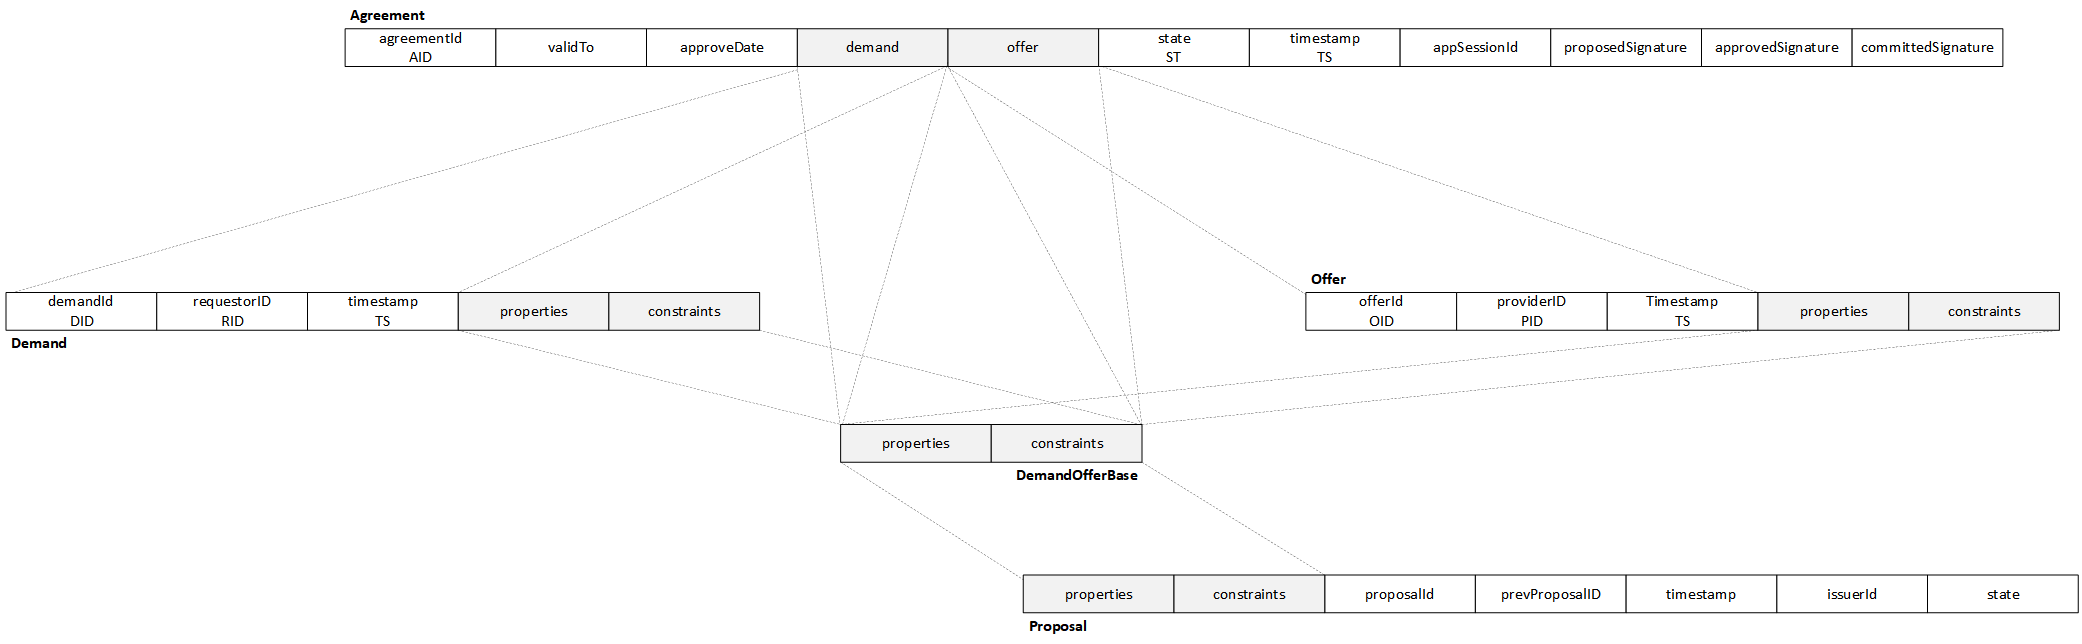
\includegraphics[width=12cm,angle=0]{./diag/Reference/MarketFrame-1-Reference.png}
	\caption{Market Objects Frame}
    \label{fig:MF1}
\end{figure}


\begin{figure}[htbp]
    \centering
    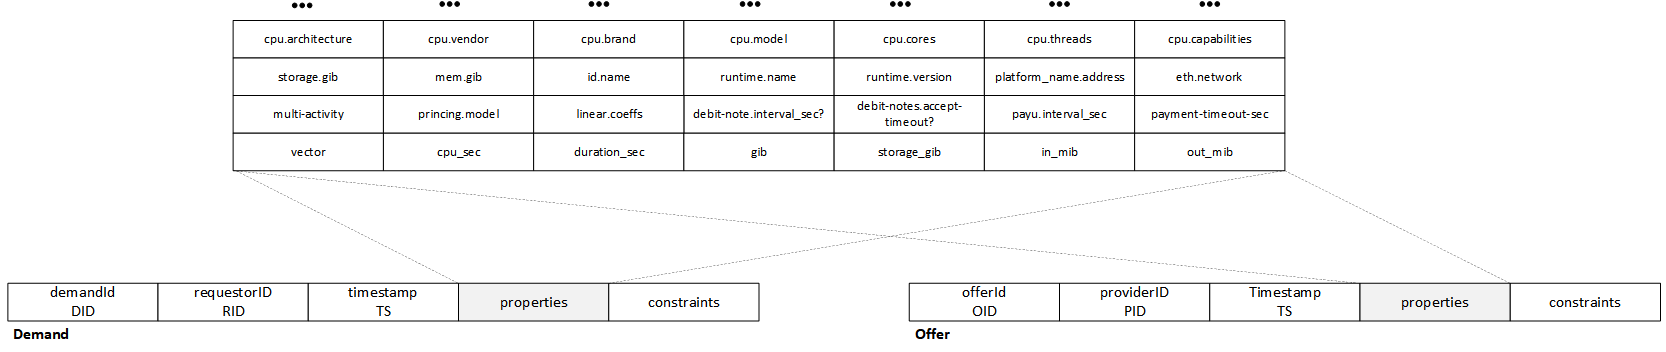
\includegraphics[width=12cm,angle=0]{./diag/Reference/MarketFrame-2-Reference.png}
	\caption{Market Objects Frame}
    \label{fig:MF2}
\end{figure}

\begin{enumerate}

\item Offer Objects

\begin{enumerate}

\item Object Description

Offer is created by Provider nodes and contains the description of the
computing resources the node has to offer, as well as any optional conditions
for their use (e.g. limiting their availability only to certain requestor nodes).

\item Object Fields

\begin{center}
\begin{tabular}{|p{3cm}|l|p{3cm}|p{3cm}|p{4cm}|} 
\hline
\rowcolor{lightgray}	Name	& MO.	& Type	& Example & 	Description \\
\hline

offerId 	& M & string & 		& Offer Identifier \\
\hline 		

providerId & M & string  & 		& Provider Node Identifier \\
\hline

timestamp	& M	& 	string(\$date-time)	& YYYY-MM-DDThh:mm:ss.sssZ	&	Time of ???  \\
\hline

properties	& M	& 	json or flat	&		&	Offer properties \\ 
\hline

constraints	& M	& 	string	&		&	Offer constraints \\ 
\hline

\end{tabular}
\end{center}

\item Object State

Stateless object

\end{enumerate}

\item Demand Objects

\begin{enumerate}

\item Object Description

Demand is created by Requestors and contains description of the
payload, including properties telling what capabilities the payload might
require (e.g. specific hardware architecture or features) and optionally other
conditions which ought to be satisfied by the provider nodes (e.g. asking only
for nodes which are located within specific country). 

%	Most of the content of the Demand is opaque for the Golem network

\item Object Fields

\begin{center}
\begin{tabular}{|p{3cm}|l|p{3cm}|p{3cm}|p{4cm}|} 
\hline
\rowcolor{lightgray}	Name	& MO.	& Type	& Example & 	Description \\
\hline

demandId 	& M & string  & 		& Demand Identifier \\
\hline 		

requestorId & M & string  & 		& Requestor Node Identifier \\
\hline

timestamp	& M	& 	string(\$date-time)	& YYYY-MM-DDThh:mm:ss.sssZ	&	Time of ???  \\
\hline

properties	& M	& 	json or flat	&		&	Demand properties \\ 
\hline

constraints	& M	& 	string	&		&	Demand constraints \\ 
\hline

\end{tabular}
\end{center}


\item Object State

Stateless object

\end{enumerate}

\item Proposal Objects

\begin{enumerate}

\item Object Description

A proposal (Proposal object) is a Demand-Offer pair (DemandOfferBase object), with a proposalId identifier and status
and a set of field elements that allow handling of the Negotiation operation. These are: the identifier of the node submitting the proposal,
the time the proposal was created, the identifier of the proposal from the other side, to which this proposal responds.

\item Object Fields

\begin{center}
\begin{tabular}{|p{3cm}|l|p{3cm}|p{3cm}|p{4cm}|} 
\hline
\rowcolor{lightgray}	Name	& MO.	& Type	& Example & 	Description \\
\hline

properties		& M	& 	json or flat		&												&	Proposal properties \\ 
\hline

constraints		& M	& 	string				&												&	Proposal constraints \\ 
\hline

proposalId		& M & 	string  			& 												& 	Proposal Identifier \\
\hline

issuerId		& M & 	string				&												& 	Issuer Node Identifier 	\\ 
\hline

state			& M & 	string(enum) 		& [Initial, Draft, Rejected, Accepted, Expired]	&  Proposal State	\\
\hline

timestamp		& M	& 	string(\$date-time)	& YYYY-MM-DDThh:mm:ss.sssZ						&	Time of ???  \\
\hline

prevProposalId 	& O & 	string				&												& 	Id of the Proposal from other side which this proposal responds to \\
\hline

\end{tabular}
\end{center}

\item Object State

(Please see Figure ~\ref{fig:PSD} on page ~\pageref{fig:PSD}).

\begin{figure}[htbp]
    \centering
    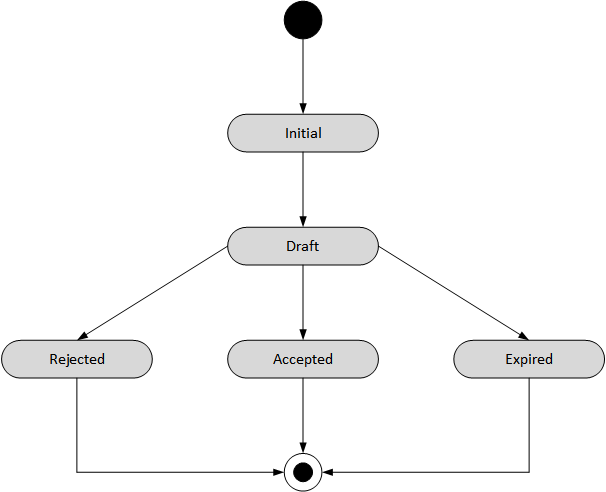
\includegraphics[width=7cm,angle=0]{./diag/Reference/ProposalState-Reference.png}
	\caption{Proposal State Diagram}
    \label{fig:PSD}
\end{figure}


\begin{center}
\begin{tabular}{|p{3cm}|p{11cm}|} 
\hline
\rowcolor{lightgray}	State	& 	Description \\
\hline

Initial 	&	proposal arrived from the market as response to subscription \\
\hline
Draft 		&	bespoke counter-proposal issued by one party directly to other party (negotiation phase) \\
\hline
Rejected 	&	reject by other party \\
\hline
Accepted 	&	promoted into the Agreement draft \\
\hline
Expired 	&	not accepted nor rejected before validity period \\
\hline

\end{tabular}
\end{center}

\end{enumerate}

\item Agreement Objects

\begin{enumerate}

\item Object Description

The Agreement object is a set of basic terms of the agreement between two parties establishing their mutual relations
in relation to the subject of the service in the market space.
The basic terms of the agreement are:

\begin{itemize}

\item Established and confirmed terms of the proposal (Proposal object) within the Negotiation operation

\item Agreement object identifier

\item Agreement object state

\item Validity date of the Agreement object circulation between the parties

\item Agreement object approval date

\item Agreement object creation date

\item Correlation/session identifier used to search for events related to the action ???

\item Proposed signature

\item Confirmed signature

\item Approved signature

\end{itemize}

\item Object Fields

\begin{center}
\begin{tabular}{|p{3cm}|l|p{3cm}|p{3cm}|p{4cm}|} 
\hline
\rowcolor{lightgray}	Name	& MO.	& Type	& Example & 	Description \\
\hline

agreementId			& M & string 				&				& 	Agreement Identifier \\
\hline

demand				& M	& object 				&				& 	Demand		\\
\hline

offer 				& M & object 				& 				& 	Offer 		\\
\hline

validTo				& M & string(\$date-time)	& YYYY-MM-DDThh:mm:ss.sssZ & End of validity period. 
																			Agreement needs to be approved, rejected or cancelled before this date; 
																			otherwise will expire. \\
\hline

approveDate			& M & string(\$date-time)	& YYYY-MM-DDThh:mm:ss.sssZ & Agreement approval timestamp \\
\hline

state 				& M & string(enum) 				&[Proposal, Pending, Cancelled, Rejected, Approved, Expired, Terminated] & Agreement State \\
\hline

timestamp			& M	& 	string(\$date-time)	& YYYY-MM-DDThh:mm:ss.sssZ	&	Time of ???  \\
\hline

appSessionId		& O &	string 				&							& 	A correlation/session identifier used for querying events related to an action 
																				where this appSessionId has been specified		\\
\hline

proposedSignature 	& O & 	string 				&							&			\\
\hline

approvedSignature 	& O & 	string 				& 							&			\\
\hline

committedSignature	& O &	string 				& 							& 			\\
\hline

\end{tabular}
\end{center}

\item Object State

(Please see Figure ~\ref{fig:ASD} on page ~\pageref{fig:ASD}).

\begin{figure}[htbp]
    \centering
    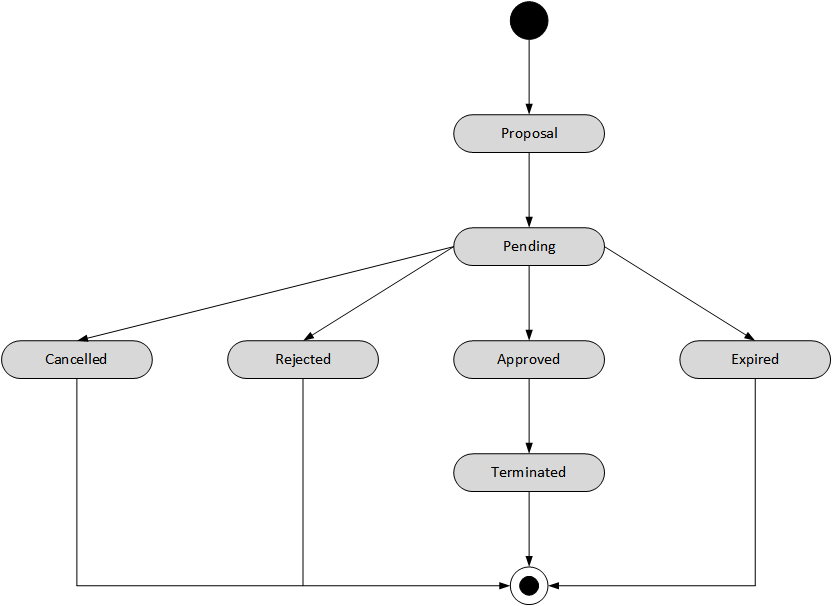
\includegraphics[width=9cm,angle=0]{./diag/Reference/AgreementState-Reference.png}
	\caption{Agreement State Diagram}
    \label{fig:ASD}
\end{figure}


\begin{center}
\begin{tabular}{|p{3cm}|p{11cm}|} 
\hline
\rowcolor{lightgray}	State	& 	Description \\
\hline

Proposal	&	newly created by a Requestor (draft based on Proposal) \\
\hline
Pending		&	confirmed by a Requestor and send to Provider for approval \\
\hline
Cancelled 	& 	by a Requestor \\
\hline
Rejected 	&	by a Provider \\
\hline
Approved 	&	by both sides \\
\hline
Expired 	&	not approved, rejected nor cancelled within validity period \\
\hline
Terminated 	&	finished after approval. \\
\hline

\end{tabular}
\end{center}

\end{enumerate}

\item DemandOfferBase Object

\begin{enumerate}

\item Object Description

The DemandOfferBase object is a temporary object that collects negotiated terms related to the service item.

\item Object Fields

\begin{center}
\begin{tabular}{|p{3cm}|l|p{3cm}|p{3cm}|p{4cm}|} 
\hline
\rowcolor{lightgray}	Name	& MO.	& Type	& Example & 	Description \\
\hline

properties	& M	& 	json or flat	&		&  Temporary Proposal properties \\ 

\hline

constraints	& M	& 	string	&		&	Temporary Proposal constraints \\ 

\hline

\end{tabular}
\end{center}

\item Object State

Stateless object

\end{enumerate}

\end{enumerate}

\break

The space is used to define interaction operations on these objects such as:

\begin{enumerate}
\item  Observation Operation

\begin{enumerate}

\item Description

The Market Observation operation is implemented by a set of Scan functions. 
These functions, together with REST API methods, allow to aggregate data from currently circulating 
offers (Offer object) and demands (Demand object).

The BeginScan() function initiates the scanning operation by accepting the filtering criteria and 
returning scanId. The results are aggregated and collected by the CollectScanResults() function.
The EndScan() function closes the data aggregation process.

The criteria for searching the Golem network market are defined using the service model description language (Golem SMDL),
where the filter syntax is based on the LDAP filter syntax. Depending on the needs, simple or complex search criteria can be defined.

(Please see Figure ~\ref{fig:MOO} on page ~\pageref{fig:MOO}).

\item Sequence Diagram

\begin{figure}[htbp]
    \centering
    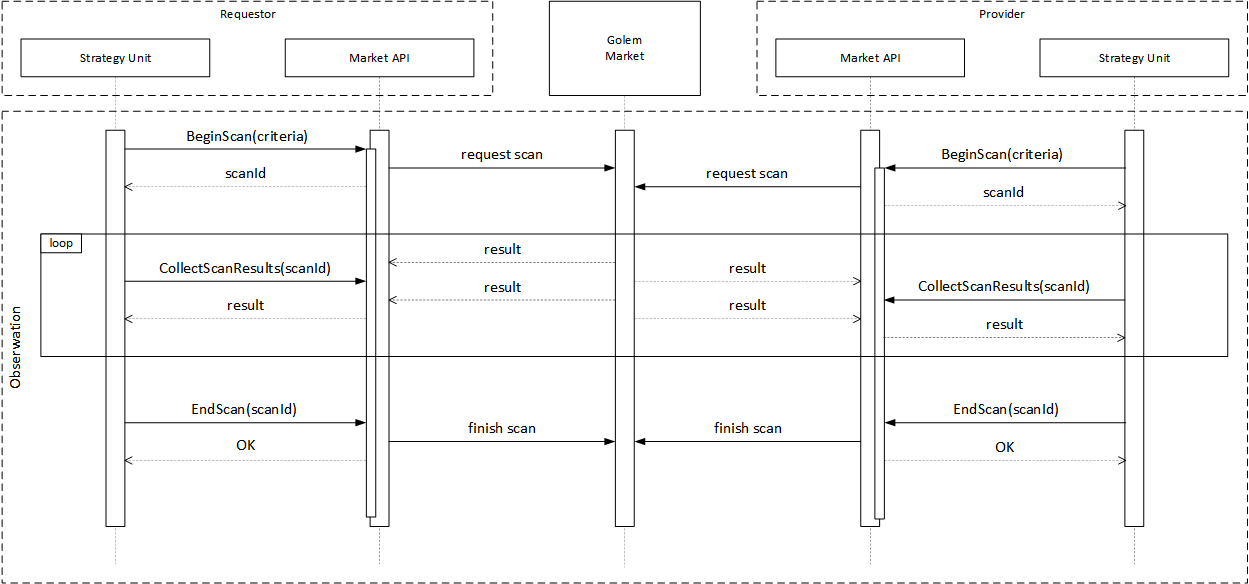
\includegraphics[width=14cm,angle=0]{./diag/Sequence/MarketObservation-B-Sequence.png}
	\caption{Market Observation Operation}
    \label{fig:MOO}
\end{figure}

\item Functions and Methods

\begin{center}
\begin{tabular}{|p{3cm}|p{7cm}|p{1.5cm}|p{4cm}|} 
\hline
\rowcolor{lightgray}	Function Name	& API Method Name	& 	Side	&	Description \\
\hline

BeginScan 				& POST /scan								&	Both	&	\\
\hline

CollectScanResult		& GET /scan/\{subscriptionId\}/events		&	Both 	& ?? subscriptionId or scanId ??	\\
\hline

EndScan 				& DELETE /scan/\{subscriptionId\}/events	&	Both 	& ?? subscriptionId or scanId ??	\\
\hline

\end{tabular}
\end{center}

\end{enumerate}

\break

\item  Discovery Operation

\begin{enumerate}

\item Description

The Discovery operation is implemented by a set of Subscribe functions. These functions, together with REST API methods, 
allow for the aggregation of data from currently circulating active offers (Offer object) and active demands (Demand object).

The Subscribe() function publishes the offer (Offer object) and demand (Demand object) on the Golem Network Market, respectively.
The aggregated results in the form of proposals (Proposal object) with matching Demand-Offer pairs are collected by the Collect() function.
The Unsubscribe() function disables the availability of offers and demands on the Golem Network Market.

The Discovery operation is the only one that involves indirect communication (e.g. via a P2P network).
The subsequent phases are direct (one-to-one)

(Please see Figure ~\ref{fig:MDO} on page ~\pageref{fig:MDO}).

\item Sequence Diagram

\begin{figure}[htbp]
    \centering
    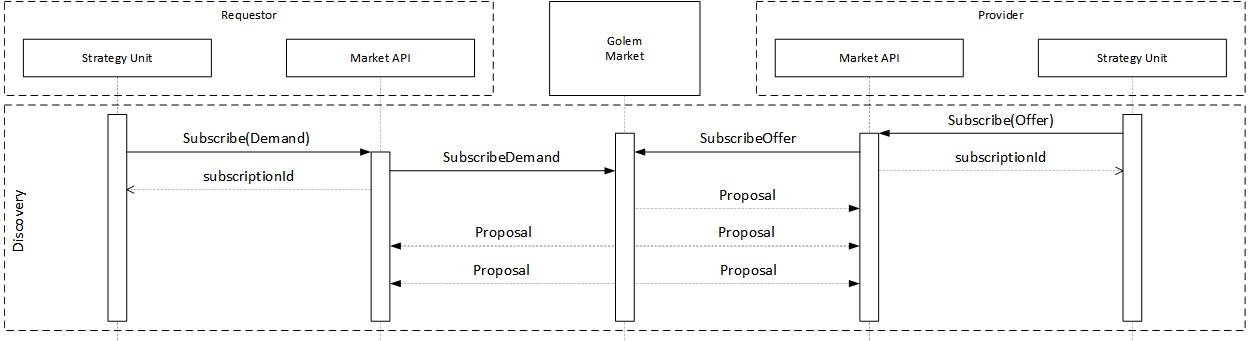
\includegraphics[width=14cm,angle=0]{./diag/Sequence/MarketDiscovery-B-Sequence.png}
	\caption{Market Discovery Operation}
    \label{fig:MDO}
\end{figure}

\item Functions and Methods

\begin{center}
\begin{tabular}{|p{3cm}|p{7cm}|p{1.5cm}|p{4cm}|} 
\hline
\rowcolor{lightgray}	Function Name	& API Method Name	& 	Side	&	Description \\
\hline

Subscribe			&	POST /offers							&	Provider	&	Publishes Provider capabilities via Offer \\
\hline

Subscribe			&	POST /demands							& 	Requestor	&	Publishes Requestor capabilities via Demand \\
\hline

Unsubscribe			&	DELETE	/offers/\{subscriptionId\}		&	Provider	&	Stop subscription for published Offer \\
\hline

Unsubscribe			&	DELETE	/demands/\{subscriptionId\}		&	Requestor	&	Stop subscription for published Demand \\
\hline	 

CollectDemands ?	&	GET	/offers/\{subscriptionId\}/events	&	Provider &	Reads Market responses to published Offer \\
\hline

CollectOffers ?		&	GET	/demands/\{subscriptionId\}/events	&	Requestor &	Reads Market responses to published Demand \\
\hline

Collect				& 	POST /offers/\{subscriptionId\}/ \newline propertyQuery/\{queryId\} & Provider & Handles dynamic property query \\
\hline

Collect				& 	POST /demands/\{subscriptionId\}/ \newline propertyQuery/\{queryId\} & Requestor & Handles dynamic property query \\
\hline 

					&	GET /offers								&	Provider	&	Fetches all active Offers which have been published by the Provider \\
\hline

					&	GET /demands							& 	Requestor	&	Fetches all active Demands which have been published by the Requestor \\
\hline	 

\end{tabular}
\end{center}

\end{enumerate}


\item  Negotiation Operation

\begin{enumerate}

\item Description

The Negotiation operation is implemented by a set of REST API functions and methods that allow for reaching a consensus between the parties
by matching offers and demands. This is done by automatic or semi-automatic exchange of documents (Offer and Demand objects)
between the parties in the form of proposals (Proposal object). 
The negotiation conditions are described by the service model description language (Golem SMDL) 
where the filter syntax is based on the LDAP filter syntax.

The Collect() function collects aggregated results in the form of proposals (Proposal object) from the data contained 
in the offer (Offer object) and in the demand (Demand object).

The CounterProposal() function In the case of the Requestor node, it creates and sends a modified version of the original demand 
(Demand object as a counterproposal) adapted to the previously received Proposal (i.e. Offer).
In the case of the Provider node, it creates and sends a modified version of the original offer (the Offer object as a counterproposal) 
adapted to the previously received proposal (i.e. Demand). The function for both cases changes the state of the Proposal object to Draft 
and returns the created proposalId. 

The RejectProposal() function effectively ends the negotiation chain - it clearly indicates
that the sender will not create another counterproposal. If the negotiations reach a consensus, 
then an agreement (the Agreement object) is generated by the CreateAgreement() function of the Agreement operation. 

The Provider node retrieves the proposal (Demand) with the given proposalId using the GetProposalDemand() method. 
The Requestor node retrieves the proposal (Offer) with the given proposalId using the GetProposalOffer() method.

(Please see Figure ~\ref{fig:MNO} on page ~\pageref{fig:MNO}).

\break

\item Sequence Diagram

\begin{figure}[htbp]
    \centering
    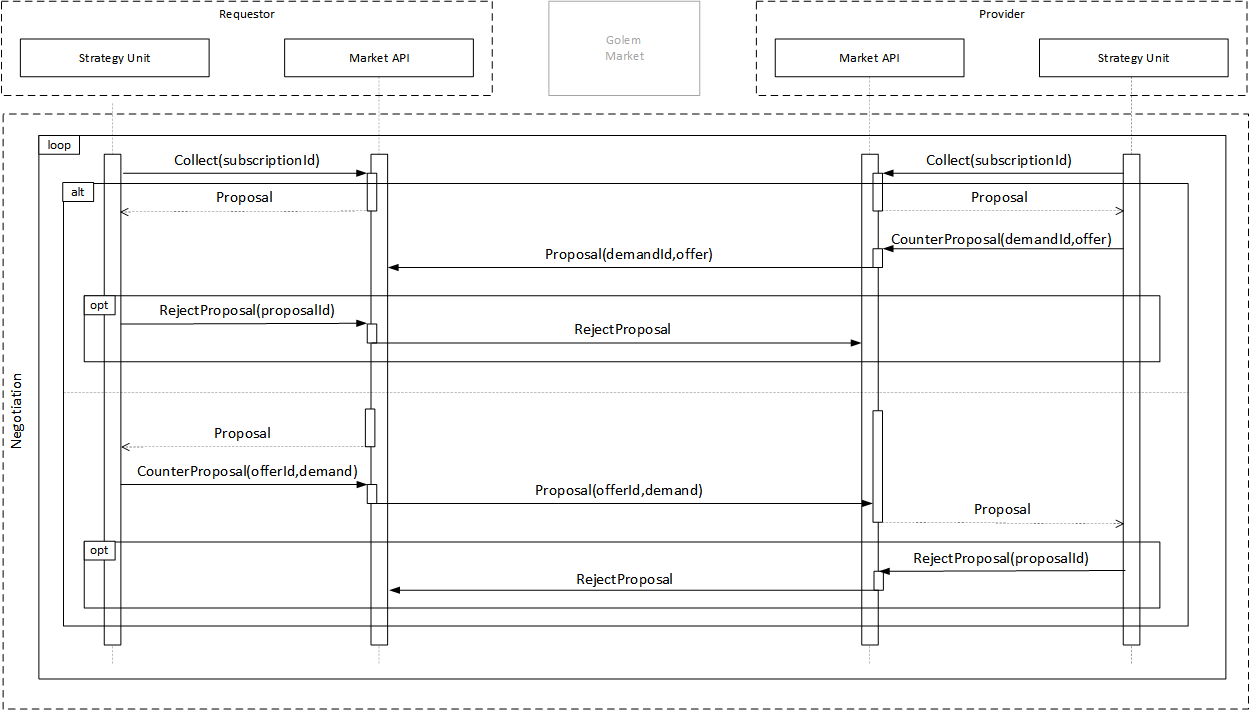
\includegraphics[width=14cm,angle=0]{./diag/Sequence/MarketNegotiation-B-Sequence.png}
	\caption{Market Negotiation Operation}
    \label{fig:MNO}
\end{figure}

\item Functions and Methods

\begin{center}
\begin{tabular}{|p{3cm}|p{7cm}|p{1.5cm}|p{4cm}|} 
\hline
\rowcolor{lightgray}	Function Name	& API Method Name	& 	Side	&	Description \\
\hline

Collect			&	GET /offers/\{subscriptionId\}/events	&	Provider	&	Reads Market responses to published Offer \\
\hline

Collect			&	GET /demands/\{subscriptionId\}/events	&	Requestor	&	Reads Market responses to published Demand \\
\hline

CounterProposal	&	POST /offers/\{subscriptionId\}/ \newline proposals/\{proposalId\}	&	Provider	&	Responds with a bespoke Offer to received Demand \\
\hline

CounterProposal	&	POST /demands/\{subscriptionId\}/ \newline proposals/\{proposalId\}	&	Requestor	&	Responds with a bespoke Demand to received Offer \\
\hline

RejectProposal	&	POST /offers/\{subscriptionId\}/ \newline proposals/\{proposalId\}/reject & Provider & Reject Proposal Demand \\
\hline

RejectProposal	&	POST /demands/\{subscriptionId\}/ \newline proposals/\{proposalId\}/reject & Requestor & Reject Proposal Offer \\
\hline

				&	GET /offers/\{subscriptionId\}/ \newline proposals/\{proposalId\}	&	Provider	&	Fetches Proposal (Demand) witch given id \\
\hline

				&	GET /demands/\{subscriptionId\}/ \newline proposals/\{proposalId\}	&	Requestor	&	Fetches Proposal (Offer) witch given id \\
\hline

\end{tabular}
\end{center}

\end{enumerate}


\item  Agreement Operation

\begin{enumerate}

\item Description

The Agreement operation is implemented by a set of REST API functions and methods that allow for the finalization of the Negotiation operation by
confirming receipt of the agreement signed by both parties (Agreement object).

The CreateAgreement() function creates an agreement (Agreement object) from the negotiated proposal (Proposal object) by the Requestor node.

The agreement created by the ConfirmAgreement() function is signed with the Applicant's signR key and sent to the Provider.

The RejectAgreement() function is used to interrupt the Agreement operation by the Provider node.

Running the RejectAgreement() function interrupts the Agreement operation, giving the Requestor node the possibility of returning the negotiation operation,
which can send a new proposal (Proposal object).

The CancelAgreement() function is used to interrupt the Agreement operation by the Requestor node.

This is possible only until the Agreement is approved or rejected by the Provider and before it expires.

The WaitForApproval() function is used to set the time to prepare resources to start the calculations as part of the Activity service operation.
This function is initialized by the Requestor node for the Provider node. After the set time has elapsed, the Requestor node can
re-call this function for the same agreement identifier (agreementId).

The ApproveAgreement() function is used to approve the agreement by the Provider node. It is used when the environment with
resources on the Provider node is ready to start the calculations by the Requestor node as part of the Activity service operation.

The TerminateAgreement() function is used to terminate the agreement in the Approved state.
The other party is notified about the decision of the calling party to terminate the "current" agreement. Available for both types of nodes.

The GetTerminateReason method is used to retrieve the reason for termination of the agreement reported during the call to the TerminateAgreement() function. Available for both types of nodes.

The AgreementEvents method is used to collect events related to the agreement (the Agreement object). These are

\begin{itemize}

\item AgreementApprovedEvent : 	indicates that the Agreement has been approved by the Provider.
								The Provider is now ready to accept the request to start the Activity
								as described in the negotiated agreement.
								The corresponding Provider approveAgreement call returns Approved after emitting this event.

\item AgreementRejectedEvent : 	indicates that the Provider has called rejectAgreement, which effectively stops the Agreement negotiation.
								The Applicant can try to return to the Negotiation phase by sending a new Proposal.

\item AgreementCancelledEvent : indicates that the Applicant has called cancelAgreement, which effectively stops the Agreement negotiation.

\item AgreementTerminatedEvent : indicates that the Agreement has been terminated by the specified party (includes a signature).

\end{itemize}

The ListAgreements method is used to retrieve information about agreements. It uses optional filters:

\begin{itemize}

\item state: [Proposal, Pending, Cancelled, Rejected, Approved, Expired, Terminated ]

\item creation date and time

\item application session identifier

\end{itemize}

The GetAgreementContent() function is used to retrieve an agreement (Agreement object) based on a given identifier (agreementId).

The ValidateAgreementContent() function is used to verify an agreement (Agreement object) sent as a byte stream.

(Please see Figure ~\ref{fig:MAO} on page ~\pageref{fig:MAO}).

\item Sequence Diagram

\begin{figure}[htbp]
    \centering
    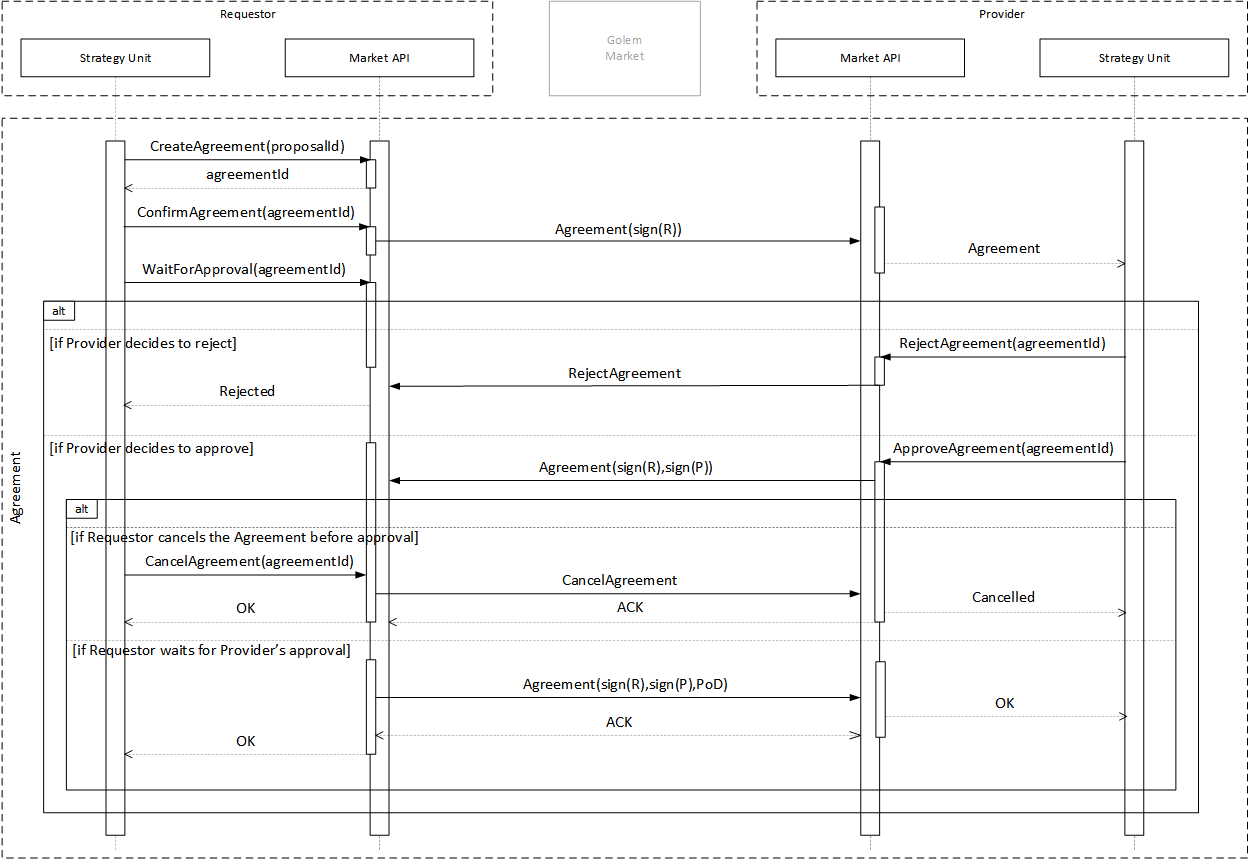
\includegraphics[width=14cm,angle=0]{./diag/Sequence/MarketAgreement-B-Sequence.png}
	\caption{Market Agreement Operation}
    \label{fig:MAO}
\end{figure}

\item Functions and Methods

\begin{table}
\footnotesize

\begin{center}
\begin{tabular}{|p{3cm}|p{7cm}|p{1.5cm}|p{4cm}|} 
\hline
\rowcolor{lightgray}	Function Name	& API Method Name							& 	Side	&	Description \\
\hline

CreateAgreement		&	POST /agreements											& Requestor	&	Creates Agreement from selected Proposal \\
\hline

					&	GET /agreements												&	Both	&	List agreements with optional filters \\
\hline

GetAgreement \newline Content	&	GET /agreements/\{agreementId\}					&	Both	&	Fetches  agreement with agreement id \\
\hline

ValidateAgreement \newline Content &												&	Both	&	Offline function for validation of agreement submitted in the form of byte stream \\
\hline

ConfirmAgreement	& POST /agreements/\{agreementId\}/ \newline terminate			& Requestor & 	Sends Agreement proposal to the Provider \\
\hline

WaitForApproval		& POST /agreements/\{agreementId\}/ \newline wait				& Requestor & 	Waits for Agreement approval by the Provider \\
\hline

CancelAgreement		& POST /agreements/\{agreementId\}/ \newline cancel				& Requestor &	Cancels Agreement	\\
\hline

TerminateAgreement	& POST /agreements/\{agreementId\}/ \newline terminate			& Both		&	Terminates approved Agreement \\
\hline

					& POST /agreements/\{agreementId\}/ \newline terminate/reason 	& Both 		& 	Gets termination reason reported when terminateAgreement operation was called \\
\hline					

					& GET /agreementEvents											& Both 		& 	Collect events related to an Agreement \\
\hline

ApproveAgreement	& POST /agreements/\{agreementId\}/ \newline Approve			& Provider	&	Approves Agreement proposed by the Requestor \\
\hline

RejectAgreement		& POST /agreements/\{agreementId\}/ \newline reject				& Provider	&	Rejects Agreement proposed by the Requestor	\\
\hline

\end{tabular}
\end{center}

\end{table}

\end{enumerate}




\end{enumerate}

%\begin{enumerate}
%    \item Service Profile
%    \item Service Protocol
%    \item Service Interface
%    \item Service Workflow
%\end{enumerate}

\subsubsubsubsection{Golem Activity Service}

This service has tools that allow the Requestor's applications and services to be launched on the Provider's computing resources,
while simultaneously measuring the use of these resources in accordance with the concluded contract in the form of an agreement. 
The measurement of the use of resources is recorded in the form of metrics in the Usage Counters Vector (UCV) object.


\begin{enumerate}
    \item Service Profile
    \item Service Protocol
    \item Service Interface
    \item Service Workflow
\end{enumerate}

\subsubsubsubsection{Golem Payment Service}

This service enables settlements between the parties based on the terms contained in the contract. 
Usage Counters Vector (UCV) objects created in the Golem Activity Service and the settlement terms included in the agreement 
are used to settle the sale-purchase item. The Usage Counters Vector (UCV) associated with the agreement and activity creates 
Activity Detail Record (ADR) objects. Settlement functions allow the ADR object to be transformed into a Debit Note (DN) object, 
where the total incremental settlement amounts for using Provider resources are included. The frequency of creating and sending 
Debit Notes objects between the parties is included in the agreement. The state of completing the use of Provider resources allows 
for the generation of an invoice summarizing the agreement between the parties. 
Payment is made via the blockchain operator. Optimization of payment transaction costs is possible by setting the terms of this operation 
in the agreement object.


\begin{enumerate}
    \item Service Profile
    \item Service Protocol
    \item Service Interface
    \item Service Workflow
\end{enumerate}

%\subsubsubsubsection{Registry and Discovery Service}

%\subsubsubsection{Golem Toolkit}

%\subsubsubsubsection{Golem Net Service API}

%\subsubsubsubsection{Golem Market Service API}

%\subsubsubsubsection{Golem Activity Service API}

%\subsubsubsubsection{Golem Payment Service API} 

%\subsubsubsubsection{Golem Rest Point}

%\subsubsection{Golem Central Net Server}

